% ============================================================================
% Mục 4.2 - Người viết: C
% ============================================================================
\subsection{Mô hình cơ sở, Ridge/Lasso và Random Forest (Phần C)}\label{sec:models-c}

Phần C xây dựng: (i) mô-đun đánh giá dùng chung \code{src/evaluate.py} để \emph{mọi} mô hình của nhóm được
chấm điểm cùng một cách; (ii) các mô hình cơ sở (baseline); (iii) hồi quy tuyến tính có điều chuẩn Ridge và
Lasso; (iv) Random Forest. Mã nguồn huấn luyện nằm ở \code{src/train_models.py}; toàn bộ thí nghiệm chạy trong
khoảng 13 phút trên CPU 12 luồng.

\subsubsection{Mô-đun đánh giá dùng chung \code{evaluate.py}}\label{sec:evaluate}

Với $n$ giờ, giá trị thực $y_i$ và dự báo $\hat{y}_i$, mô-đun tính sáu chỉ số:
\begin{align}
\mathrm{MAE} &= \frac1n\sum_{i=1}^n |y_i-\hat y_i|, &
\mathrm{RMSE} &= \sqrt{\frac1n\sum_{i=1}^n (y_i-\hat y_i)^2},\\
\mathrm{MAPE} &= \frac{100}{n}\sum_{i=1}^n \left|\frac{y_i-\hat y_i}{y_i}\right|, &
\mathrm{sMAPE} &= \frac{100}{n}\sum_{i=1}^n \frac{|y_i-\hat y_i|}{(|y_i|+|\hat y_i|)/2},\\
R^2 &= 1-\frac{\sum_i (y_i-\hat y_i)^2}{\sum_i (y_i-\bar y)^2}, &
\mathrm{MaxAE} &= \max_i |y_i-\hat y_i|.
\end{align}

\paragraph{Lý do chọn chỉ số.} \textbf{MAE} (đơn vị MW) dễ diễn giải với người vận hành và là tiêu chí
chọn siêu tham số; \textbf{RMSE} phạt nặng các giờ sai lớn --- vốn gây tốn kém nhất (huy động dự phòng);
\textbf{MAPE} không phụ thuộc thang đo, dùng được vì phụ tải luôn $\geq 18\,000$~MW nên không có vấn đề chia
cho số gần 0~\cite{hyndman2006accuracy}; \textbf{MaxAE} cho biết giờ tệ nhất.

\paragraph{Thiết kế.} Mô-đun gồm:
\begin{itemize}
  \item Các hàm chỉ số thuần NumPy, kiểm tra đầu vào (khác kích thước, NaN/inf, MAPE khi $y=0$ đều báo lỗi
        thay vì âm thầm trả về số sai).
  \item Lớp \code{ResultsLog} tích lũy các dòng (mô hình, tập, chỉ số) và xuất bảng/CSV --- phần D và E chỉ
        cần gọi \code{log.add(...)} là có kết quả cùng định dạng với \cref{tab:main-results}.
  \item Các hàm chẩn đoán: \code{error_by_group} (MAE theo giờ/thứ/tháng địa phương), \code{plot_forecast},
        \code{plot_residuals}, \code{plot_metric_bars}.
\end{itemize}

\begin{lstlisting}[caption={Cách dùng \code{evaluate.py} cho bất kỳ mô hình nào.},label={lst:evaluate}]
from evaluate import ResultsLog
log = ResultsLog()
log.add("Random Forest", "test", test[TARGET], rf.predict(test[cols]), family="tree")
log.to_frame()            # DataFrame: model, split, MAE, RMSE, MAPE, sMAPE, R2, MaxAE
log.save(Path("results/metrics.csv"))
\end{lstlisting}

\subsubsection{Giao thức thực nghiệm}\label{sec:protocol}

Mọi mô hình tuân theo cùng một giao thức, nhằm tránh chọn siêu tham số dựa trên tập test:
\begin{enumerate}
  \item \textbf{Tinh chỉnh}: fit trên \emph{train} (23\,872 giờ sau khi bỏ 4 tuần khởi động lag), chọn cấu hình
        có MAE nhỏ nhất trên \emph{validation} (5\,260 giờ).
  \item \textbf{Đánh giá cuối}: fit lại cấu hình đã chọn trên \emph{train + validation}, chấm điểm \emph{một lần}
        trên \emph{test} (5\,260 giờ, 26/05--31/12/2018).
\end{enumerate}
Không dùng k-fold ngẫu nhiên vì sẽ trộn tương lai vào tập huấn luyện~\cite{bergmeir2012cv}. Fit lại trên
train+val giúp mô hình thấy dữ liệu gần tập test nhất (mùa đông 2017--2018), điều quan trọng với chuỗi có xu hướng.

\subsubsection{Các mô hình cơ sở}\label{sec:baselines}

Mô hình cơ sở cho biết một mô hình học máy có thực sự ``học'' được gì hay không~\cite{hyndman2021fpp3}:
\begin{itemize}
  \item \textbf{Ngây thơ theo ngày}: $\hat y_t = y_{t-24}$ (cùng giờ hôm qua).
  \item \textbf{Ngây thơ theo mùa (tuần)}: $\hat y_t = y_{t-168}$ (cùng giờ, cùng thứ tuần trước) --- xử lý
        được chuyển tiếp cuối tuần/đầu tuần.
  \item \textbf{Trung bình 4 tuần}: $\hat y_t = \frac14\sum_{k=1}^4 y_{t-168k}$ --- giảm nhiễu của một tuần đơn lẻ.
  \item \textbf{Dự báo của TSO} (\code{total load forecast}, \emph{chỉ để tham chiếu}): đây là dự báo do đơn vị
        vận hành lưới công bố, có dùng thông tin mà nhóm không có. Như phân tích ở \cref{sec:horizon}, sai số
        của nó tương đương mô hình dự báo trước 1 giờ, nên \textbf{không phải đối thủ công bằng} cho bài toán
        $h=24$; nó cho biết giới hạn trên thực tế.
\end{itemize}
Các baseline không cần huấn luyện nên chúng được tính trực tiếp từ các cột lag của \cref{sec:feat-lag}.

\subsubsection{Ridge và Lasso}\label{sec:linear}

Hồi quy tuyến tính với điều chuẩn $\ell_2$ (Ridge~\cite{hoerl1970ridge}) và $\ell_1$ (Lasso~\cite{tibshirani1996lasso}):
\begin{align}
\hat\beta^{\text{Ridge}} &= \arg\min_\beta\ \|y - X\beta\|_2^2 + \alpha\|\beta\|_2^2,\\
\hat\beta^{\text{Lasso}} &= \arg\min_\beta\ \tfrac{1}{2n}\|y - X\beta\|_2^2 + \alpha\|\beta\|_1.
\end{align}
Các đặc trưng lag tương quan rất mạnh với nhau (\code{lag_24}, \code{roll_mean_24}, \code{roll_max_24},\dots),
nên OLS thuần sẽ có hệ số không ổn định; Ridge co các hệ số về 0 để ổn định, còn Lasso có thể đưa hẳn hệ số về
0, tức tự chọn đặc trưng.

\paragraph{Tiền xử lý trong pipeline.} Mô hình tuyến tính không tự học được tương tác, nên phần C dùng
\code{ColumnTransformer} gồm: \code{StandardScaler} cho 35 biến số và \code{OneHotEncoder} (bỏ mức đầu) cho
4 biến phân loại: \code{cal_hour}, \code{cal_dayofweek}, \code{cal_month} và tương tác
\code{cal_hour}~$\times$~\code{cal_is_offday} (48 mức) --- cho phép hình dạng phụ tải trong ngày khác nhau giữa
ngày làm việc và ngày nghỉ. Tổng cộng 123 hệ số. Vì scaler nằm trong \code{Pipeline}, nó chỉ học trung bình/độ
lệch chuẩn từ dữ liệu được \code{fit}.

\paragraph{Tinh chỉnh $\alpha$.} Ridge: 13 giá trị $\alpha\in[10^{-2},10^{4}]$ (thang log); Lasso: 8 giá trị
$\alpha\in[10^{-1},10^{2.5}]$. Kết quả ở \cref{fig:tuning-linear}: chọn $\alpha^{\text{Ridge}}=100$ (MAE val
1\,856~MW) và $\alpha^{\text{Lasso}}=3.16$ (1\,850~MW). Đường cong khá phẳng với $\alpha$ nhỏ, cho thấy
điều chuẩn chỉ cải thiện nhẹ (~15~MW); $\alpha$ quá lớn làm mô hình underfit rõ rệt. Lasso giữ lại
\textbf{82/123} hệ số khác 0; các hệ số lớn nhất là các mức giờ tối (20--22h), \code{lag_24}, các tương tác
giờ~$\times$~ngày nghỉ và tháng 7 (điều hòa mùa hè) --- phù hợp trực giác.

\begin{figure}[H]
\centering
\begin{subfigure}{0.49\linewidth}
  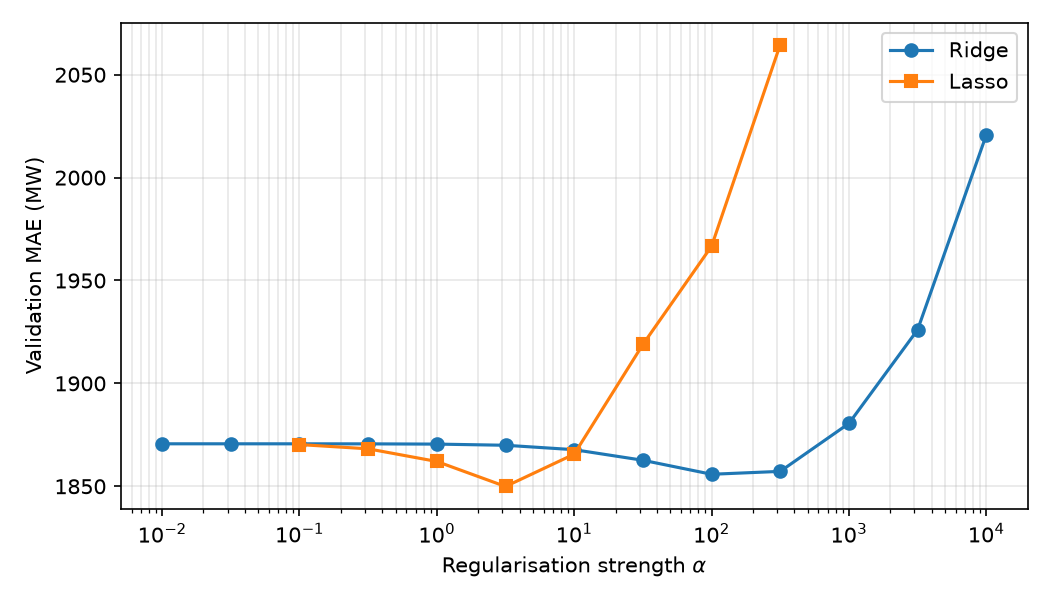
\includegraphics[width=\linewidth]{c_tuning_linear.png}
  \caption{Ridge / Lasso theo $\alpha$.}\label{fig:tuning-linear}
\end{subfigure}\hfill
\begin{subfigure}{0.49\linewidth}
  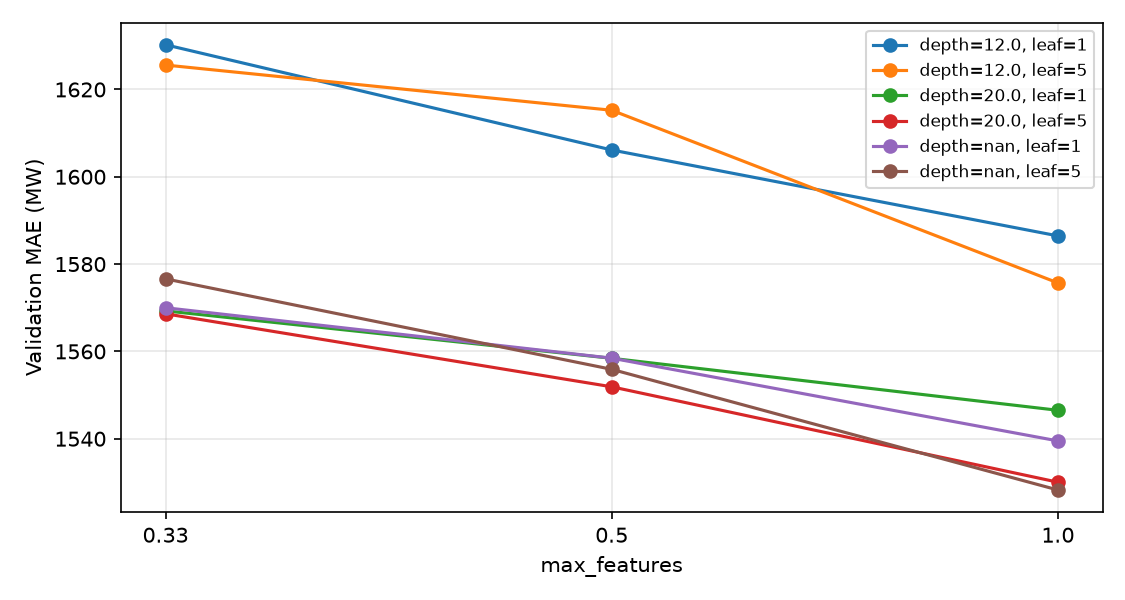
\includegraphics[width=\linewidth]{c_tuning_rf.png}
  \caption{Random Forest theo lưới siêu tham số.}\label{fig:tuning-rf}
\end{subfigure}
\caption{Đường cong tinh chỉnh trên tập validation (MAE).}
\end{figure}

\subsubsection{Random Forest}\label{sec:rf}

Random Forest~\cite{breiman2001random} là trung bình của $B$ cây hồi quy, mỗi cây học trên một mẫu bootstrap và
tại mỗi nút chỉ xét ngẫu nhiên \code{max_features} đặc trưng:
\begin{equation}
\hat y(x) = \frac1B\sum_{b=1}^B T_b(x).
\end{equation}
Mô hình tự học tương tác (giờ~$\times$~ngày nghỉ~$\times$~nhiệt độ) và quan hệ phi tuyến chữ U mà không cần
thiết kế thủ công, không cần chuẩn hóa, và việc lấy trung bình giảm phương sai của từng cây.

\paragraph{Tinh chỉnh.} Lưới 18 cấu hình (200 cây mỗi cấu hình):
\code{max_depth}~$\in\{12, 20, \text{None}\}$, \code{min_samples_leaf}~$\in\{1,5\}$,
\code{max_features}~$\in\{0.33, 0.5, 1.0\}$. Cấu hình tốt nhất: \code{max_depth=None},
\code{min_samples_leaf=5}, \code{max_features=1.0} (MAE val 1\,528~MW). \Cref{fig:tuning-rf} cho thấy: cây sâu
hơn luôn tốt hơn (độ sâu 12 bị underfit), \code{min_samples_leaf=5} làm mượt lá và tốt hơn 1 một chút, và
\code{max_features=1.0} (tức bagging thuần) tốt nhất --- vì có ít đặc trưng thực sự mạnh (\code{lag_24},
\code{cal_hour}), buộc cây bỏ qua chúng ở một nút làm giảm chất lượng nhiều hơn lợi ích giải tương quan.
Mô hình cuối dùng 500 cây.

\subsubsection{Kết quả}\label{sec:compare-c}

\begin{table}[H]
\centering
\caption{Kết quả dự báo trước 24 giờ. Validation: mô hình fit trên train. Test: fit trên train+val.
In đậm: tốt nhất trong các mô hình của nhóm.}\label{tab:main-results}
\small
\begin{tabular}{lrrrrrrrr}
\toprule
& \multicolumn{4}{c}{Validation} & \multicolumn{4}{c}{Test}\\
\cmidrule(lr){2-5}\cmidrule(lr){6-9}
Mô hình & MAE & RMSE & MAPE & $R^2$ & MAE & RMSE & MAPE & $R^2$\\
\midrule
Ngây thơ $y_{t-24}$ & 2\,429 & 3\,507 & 8.43 & 0.445 & 2\,533 & 3\,622 & 8.76 & 0.378\\
Ngây thơ $y_{t-168}$ & 2\,571 & 3\,663 & 8.87 & 0.394 & 2\,589 & 3\,818 & 8.96 & 0.308\\
Trung bình 4 tuần & 2\,245 & 3\,019 & 7.85 & 0.589 & 2\,223 & 3\,029 & 7.68 & 0.565\\
Ridge ($\alpha=100$) & 1\,856 & 2\,513 & 6.39 & 0.715 & 1\,788 & 2\,520 & 6.14 & 0.699\\
Lasso ($\alpha=3.16$) & 1\,850 & 2\,507 & 6.37 & 0.716 & 1\,787 & 2\,524 & 6.14 & 0.698\\
\textbf{Random Forest} & \textbf{1\,527} & \textbf{2\,269} & \textbf{5.24} & \textbf{0.768} & \textbf{1\,530} & \textbf{2\,355} & \textbf{5.22} & \textbf{0.737}\\
\midrule
\textit{Dự báo TSO (tham chiếu)} & \textit{304} & \textit{451} & \textit{1.05} & \textit{0.991} & \textit{255} & \textit{342} & \textit{0.87} & \textit{0.994}\\
\bottomrule
\end{tabular}
\\[2pt]\footnotesize MAE, RMSE tính bằng MW; MAPE tính bằng \%. File đầy đủ (gồm sMAPE, MaxAE): \code{results/metrics.csv}.
\end{table}

\begin{figure}[H]
\centering
\begin{subfigure}{0.49\linewidth}
  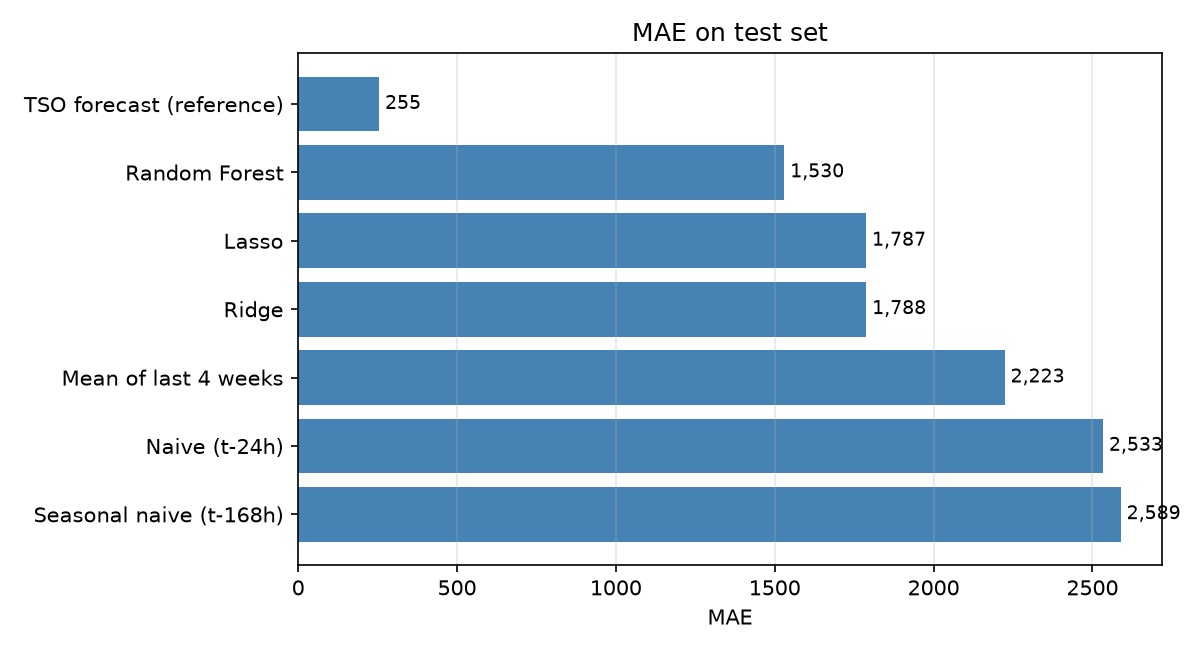
\includegraphics[width=\linewidth]{c_mae_test.png}
  \caption{MAE trên tập test.}
\end{subfigure}\hfill
\begin{subfigure}{0.49\linewidth}
  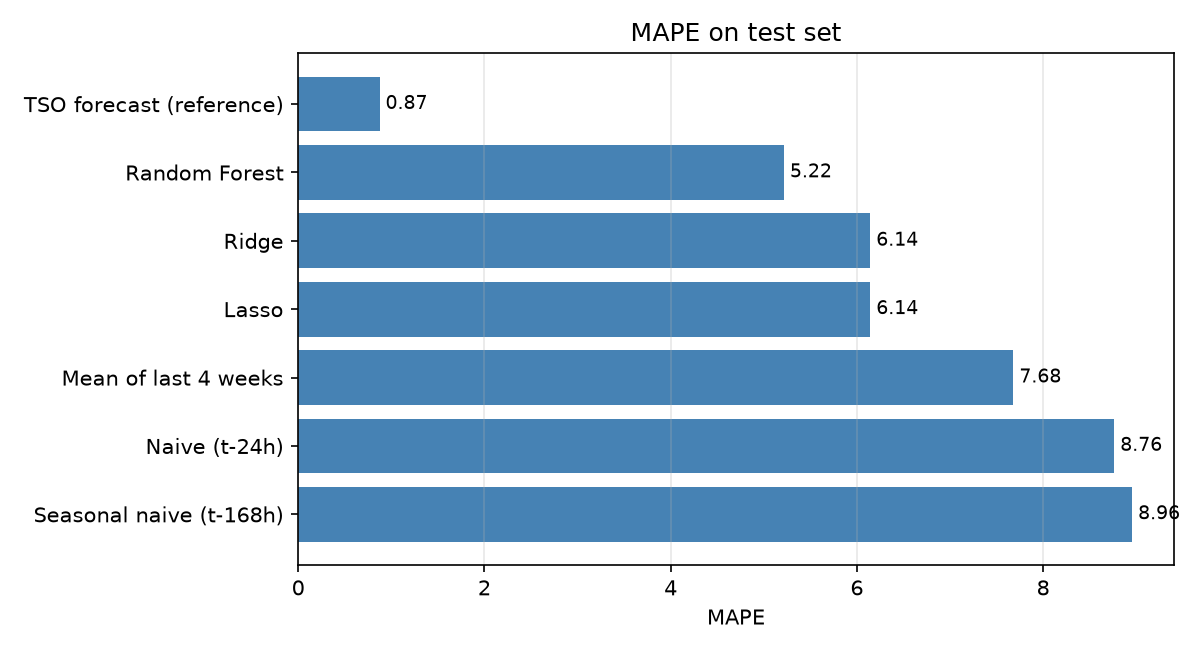
\includegraphics[width=\linewidth]{c_mape_test.png}
  \caption{MAPE trên tập test.}
\end{subfigure}
\caption{So sánh các mô hình của phần C trên tập test.}\label{fig:bars}
\end{figure}

\paragraph{Nhận xét chính.}
\begin{enumerate}
  \item \textbf{Mọi mô hình học máy đều vượt baseline.} Random Forest giảm MAE 39.6\% so với $y_{t-24}$ và
        31.2\% so với baseline tốt nhất (trung bình 4 tuần). Ridge/Lasso giảm 19.6\% so với baseline tốt nhất.
  \item \textbf{Random Forest tốt hơn tuyến tính 14.4\% MAE} nhờ học được tương tác và quan hệ phi tuyến.
        Khoảng cách RMSE nhỏ hơn (6.6\%), nghĩa là RF chủ yếu tốt hơn ở các giờ ``bình thường''; cả hai đều
        sai lớn ở các ngày bất thường.
  \item \textbf{Ridge và Lasso gần như như nhau} (chênh lệch $<1$~MW trên test): với 23\,872 mẫu và 123 hệ số,
        điều chuẩn chỉ đóng vai trò nhỏ; ưu điểm của Lasso là mô hình thưa hơn (82 hệ số).
  \item \textbf{Tổng quát hóa ổn định}: sai số val và test gần nhau (RF: 1\,527 vs 1\,530~MW), cho thấy giao
        thức tinh chỉnh không overfit tập validation. $R^2$ test thấp hơn val chủ yếu do phương sai của tập
        test nhỏ hơn (mùa hè--thu), không phải do sai số tăng.
  \item \textbf{Ngây thơ tuần kém hơn ngây thơ ngày}, trái với dữ liệu phụ tải thông thường --- một hệ quả của
        tính mùa vụ tuần yếu đã nêu ở \cref{sec:data-quirk}.
\end{enumerate}

\subsubsection{Phân tích sai số}\label{sec:error-analysis}

\begin{figure}[H]
\centering
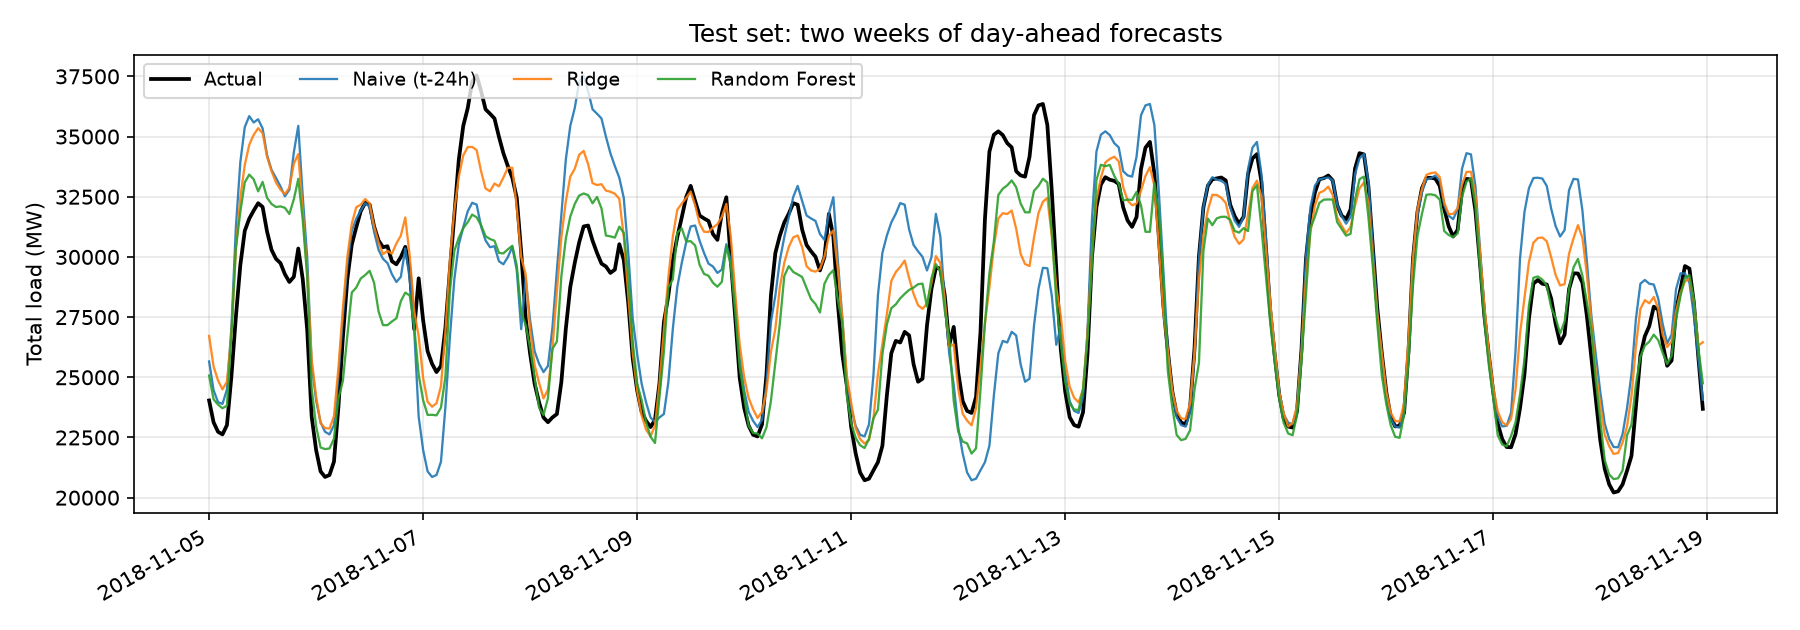
\includegraphics[width=\linewidth]{c_forecast_2weeks.png}
\caption{Hai tuần dự báo trên tập test, từ ngày 5 đến ngày 19 tháng 11 năm 2018.}\label{fig:forecast}
\end{figure}

\Cref{fig:forecast} cho thấy cả ba mô hình bám tốt hình dạng ngày (đáy đêm, đỉnh sáng và tối). Mô hình ngây
thơ ``trễ một ngày'' rõ rệt: khi một ngày có phụ tải bất thường (12/11), nó lặp lại bất thường đó vào ngày hôm
sau. Ridge và đặc biệt Random Forest giảm đáng kể lỗi lặp này nhờ kết hợp lag với lịch và trung bình nhiều tuần,
nhưng không thể đoán trước một ngày bất thường như 07/11 hay 12/11.

\begin{figure}[H]
\centering
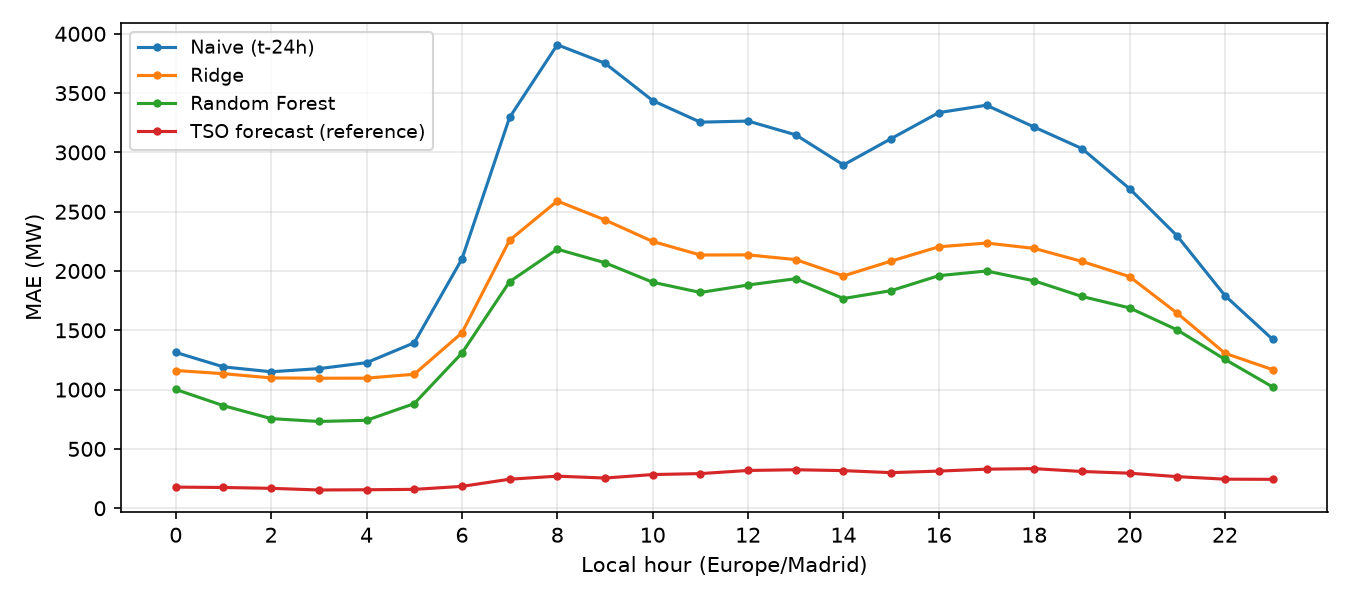
\includegraphics[width=0.85\linewidth]{c_mae_by_hour.png}
\caption{MAE theo giờ địa phương trên tập test.}\label{fig:mae-hour}
\end{figure}

\paragraph{Theo giờ (\cref{fig:mae-hour}).} Sai số nhỏ nhất vào 2--5h sáng (phụ tải nền ổn định, RF
$\approx 750$~MW) và lớn nhất vào 8h sáng (RF $\approx 2\,200$~MW) --- giờ tăng tải buổi sáng, nhạy với
việc ngày đó là ngày làm việc hay nghỉ. RF tốt hơn Ridge ở mọi giờ, rõ nhất vào ban đêm.

\paragraph{Theo thứ.} MAE test của RF thấp nhất vào Thứ Tư (1\,274~MW) và Thứ Sáu (1\,314~MW), cao nhất vào
Thứ Bảy (1\,723~MW) và Chủ Nhật (1\,988~MW). Baseline $y_{t-24}$ đặc biệt tệ vào Thứ Hai (4\,396~MW) vì dùng
phụ tải Chủ Nhật; RF giảm lỗi Thứ Hai xuống 1\,469~MW ($-67\%$) nhờ biến \code{cal_is_offday} và lag tuần.

\paragraph{Các giờ sai lớn nhất} tập trung vào một số ngày cuối tuần có phụ tải ở mức ngày làm việc (02/06,
01/09, 01/12/2018: sai tới 10\,000~MW) và Giáng Sinh 25/12 (dự báo cao hơn thực tế $\approx 9\,600$~MW lúc 8h).
Ngày lễ chỉ xuất hiện 2--3 lần mỗi năm trong train nên mô hình học được hiệu ứng ngày lễ chưa đủ mạnh.

\begin{figure}[H]
\centering
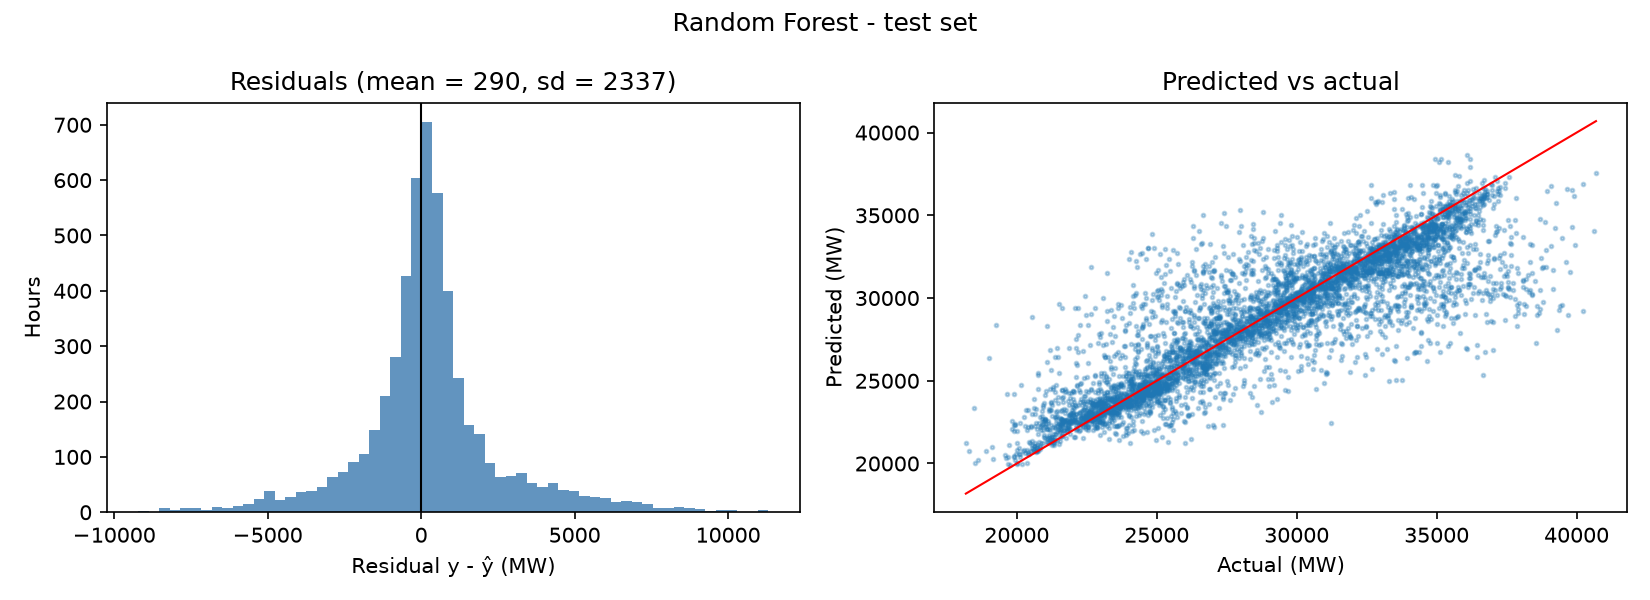
\includegraphics[width=0.95\linewidth]{c_residuals_rf.png}
\caption{Phần dư của Random Forest trên tập test.}\label{fig:residuals}
\end{figure}

\Cref{fig:residuals} cho thấy phần dư tập trung quanh 0 nhưng có đuôi dày ở cả hai phía --- tương ứng với các
ngày bất thường nói trên --- và mô hình có xu hướng ``co về trung bình'' ở các giờ phụ tải rất cao
(điểm nằm dưới đường chéo ở góc phải), một đặc điểm đã biết của Random Forest: dự báo là trung bình các lá nên
không ngoại suy vượt khoảng giá trị đã thấy.

\subsubsection{Hạn chế và đề xuất cho phần D, E}
\begin{itemize}
  \item Random Forest là mô hình tốt nhất của phần C và là \textbf{mốc để phần D (LightGBM/XGBoost) so sánh};
        boosting có thể giảm thêm thiên lệch ở các giờ cao tải.
  \item Dự báo TSO vẫn tốt hơn nhiều; một phần do TSO có thông tin cập nhật trong ngày. Với $h=1$, RF đạt MAPE
        1.07\% (\cref{tab:horizon}), ngang TSO.
  \item Cải tiến khả thi: đặc trưng ngày lễ vùng (Catalonia, Madrid, \dots), ``ngày sau lễ'', trọng số theo dân số
        cho thời tiết 5 thành phố, và dự báo xác suất (khoảng tin cậy) thay vì điểm.
\end{itemize}
